\section{\Tool{}'s design}%
\label{sec:design}

We now discuss \tool{}'s design by first laying out our trust assumptions and by
providing an informal design overview (\S~\ref{sec:assumptions-overview}),
followed by a discussion of the two major aspects of our tool kit: the
reproducible build system (\S~\ref{sec:build-system}) and \tool{}
itself~(\S~\ref{sec:framework}).

\subsection{Trust assumptions and design overview}%
\label{sec:assumptions-overview}

Our setting has three participants that make the following trust assumptions:
%
The \emph{service provider} runs a service for clients.  As part of its
operations, the service provider wants to process sensitive client information.

The \emph{client} is a user of the service provider.  It does not trust the
service provider with its sensitive information and demands verifiable
guarantees that the service provider will never see the client's sensitive
information in plain text.

The \emph{enclave provider} makes available enclaves to the service provider.
Both the client and the service provider trust that the enclave provider's
enclaves have the advertised security attributes of integrity, confidentiality,
and verifiability.

We begin with an informal overview of \tool{} to provide intuition.  Subsequent
sections are going to elaborate on the details.  The life cycle of an enclave
application that uses \tool{} involves six steps:

\ding{202} The service provider wants to run an existing service in an enclave.
Assuming that the service builds reproducibly, the service provider then
publishes the service's source code for its clients to audit.

\ding{203} The service provider bundles its service with \tool{} and launches
the enclave, which is now ready to receive incoming connections.

\ding{204} Users audit the service's (freely available) source code.  Once a
user is convinced that the code is free of security bugs, she compiles the
service using the deterministic build system, which results in an image
checksum.

\ding{205} The client establishes an end-to-end encrypted network connection
with the enclave.  Right \emph{after} establishing the secure channel but
\emph{before} revealing any sensitive information, the client provides a nonce
and asks the enclave for an attestation document.

\ding{206} The enclave receives the nonce and asks its hypervisor to generate an
attestation document that contains the client-provided nonce \emph{and} the
public key that the enclave uses to establish the secure channel.  The enclave
returns the resulting attestation document (which contains the image checksum)
to the client.

\ding{207} The client performs various checks (see \S~\ref{sec:attestation} for
details) and trusts the enclave if all checks pass.  The client is then
convinced that it's communicating with the code that the user audited in the
previous steps and is willing to reveal her sensitive information to the
enclave.

\subsection{Enabling reproducible builds}%
\label{sec:build-system}

Once a user audited the service's code, she compiles the code to obtain the PCR0
value (cf.~Table~\ref{tab:pcr}).\footnote{We use the terms ``PCR0 value'' and
``image ID'' interchangeably.}  Crucially, we need a \emph{deterministic
mapping} between the code and its corresponding image ID because the service
provider and clients must agree on the image ID that's running in the enclave.
Docker by itself does not provide a deterministic mapping because---among other
things---Docker records timestamps in its build process, causing subsequent
builds of identical code to result in different image IDs.\footnote{In essence,
a Docker image is an archive of a file system.  A Docker image is reproducible
when separate build processes arrive at the exact same file system, including
meta data like timestamps.}  To obtain reproducible builds, we take advantage of
kaniko~\cite{kaniko}, which is straightforward to integrate into existing
Docker-based workflows.  Kaniko's purpose is to build container images from a
Dockerfile while itself in a container, but we use kaniko because it can do so
reproducibly.  As long as the client and service provider use the same source
code, kaniko version, and compiler, they can build identical images---even when
compiling the code on different platforms, like macOS and Linux.  Equipped with
a locally-generated PCR0 value (henceforth simply called ``image ID''), the
client is now ready to interact with the enclave.

\subsection{\Tool{}'s components}%
\label{sec:framework}

Having discussed how the client and service provider can independently arrive at
identical image IDs, we now turn to \tool{}'s architecture.  The
following sections discuss how \tool{}
communicates securely with the outside world (\S~\ref{sec:networking});
how we facilitate remote attestation (\S~\ref{sec:attestation});
how enclaves can share their key material to allow for horizontal scaling (\S~\ref{sec:sync});
how to thwart side-channel attacks (\S~\ref{sec:side-channels}); and
how to ingest secrets (\S~\ref{sec:secrets}).
Appendix~\ref{sec:example} provides an example of a simple enclave application.

\subsubsection{Enabling seamless and secure networking}%
\label{sec:networking}

\begin{figure}[t]
  \centering
  \begin{tikzpicture}[node distance=20pt]
	\node [draw,
           label=EC2 parent,
           minimum height=100pt,
           align=center,
           minimum width=80pt] (ec2) {};
	\node [draw,
           label=Enclave,
           right=0pt of ec2,
           fill=black!10,
           minimum height=100pt,
           minimum width=80pt] (enclave) {};
           
    \node [draw,
           below=0pt of enclave.south west,
           minimum width=160pt] (hypervisor) {Hypervisor};
	   
	\node [draw,
           align=center,
           minimum height=25pt,
           yshift=-5pt,
           above=of ec2.south] (viproxy) {TCP proxy};

	\node [draw,
           align=center,
           yshift=5pt,
           below=of ec2.north] (socks) {SOCKS\\proxy};
  
	\node[draw,
          align=center,
          fill=white,
          minimum height=25pt,
          yshift=-5pt,
          above=of enclave.south] (app) {Application};
	      
	\node [draw,
           minimum height=16pt,
           yshift=35pt,
           left=of ec2.west] (backend) {Back end};

    \node [draw,
           below=of backend] (letsencrypt) {Let's Encrypt};

    \node [draw,
           below=of letsencrypt,
           minimum height=16pt] (client) {Client};

    \node [right, align=center, rotate=90] at (enclave.west) {\footnotesize \color{gray} VSOCK\\\footnotesize \color{gray} interface};

    % Application asks the hypervisor for randomness.
    \draw[-latex] (app.south) -- ([xshift=40pt]hypervisor.north)
        node [midway, fill=white, circle, inner sep=0pt] {\ding{202}};

    % Application talking to Let's Encrypt.
    \draw[-latex, densely dotted] ([yshift=10pt]app.west) -- ([yshift=10pt]viproxy.east)
        node [midway, fill=white, circle, inner sep=0pt] {\ding{203}};
    \draw[-latex, densely dotted] ([xshift=-3pt]viproxy.north) -- ([xshift=-3pt]socks.south);
    \draw[-latex, densely dotted] ([yshift=-3pt]socks.west) -- ([yshift=3pt]letsencrypt.east);

    % Let's encrypt probing Application.
    \draw[-latex, densely dashdotted] ([yshift=-3pt]letsencrypt.east) -- ([yshift=3pt]viproxy.west)
        node [midway, fill=white, circle, inner sep=0pt] {\ding{204}};
    \draw[-latex, densely dashdotted] ([yshift=3pt]viproxy.east) -- ([yshift=3pt]app.west);

    % Clients talking to the application.
    \draw[-latex] (client.east) -- ([yshift=-3pt]viproxy.west)
        node [midway, fill=white, circle, inner sep=0pt] {\ding{205}};
    \draw[-latex] ([yshift=-3pt]viproxy.east) -- ([yshift=-3pt]app.west);
    
    % Application talking to backend.
	\draw[-latex, densely dashed] ([yshift=-10pt]app.west) -- ([yshift=-10pt]viproxy.east)
	    node [midway, fill=white, circle, inner sep=0pt] {\ding{206}};
	\draw[-latex, densely dashed] ([xshift=3pt]viproxy.north) -- ([xshift=3pt]socks.south);
	\draw[-latex, densely dashed] ([yshift=3pt]socks.west) -- (backend.east);
\end{tikzpicture}
  \caption{An architectural diagram illustrating the data flow as \tool{} first
    boots and as clients talk to the enclave application.}%
  \label{fig:networking}
\end{figure}

Nitro Enclaves have no networking interface.  Their only way to talk to the
outside world is a VSOCK interface connected to the EC2 host.  \Tool{}
works around this limitation by creating a TAP interface~\cite{tun-tap} inside
the enclave as illustrated in Figure~\ref{fig:networking}.  The TAP interface is
a virtual networking interface that acts as a network bridge between the enclave
and the EC2 host.  This interface routes traffic to a cooperating proxy
application running on the EC2 host, which provides the enclave application with
seamless Internet connectivity for both IPv4 and IPv6.  The proxy supports port
forwarding to both \tool{} and the enclave application (which are independent
processes), allowing clients to talk to either directly.  \Tool{} supports two
modes for the enclave application to receive connections from clients:

{\bf Reverse proxy}: \Tool{} acts as an HTTP reverse proxy and forwards incoming
HTTP requests to the enclave application.  \Tool{} terminates the TLS
connection, meaning that the enclave application can use plain HTTP.  This mode
is only applicable if the enclave application exposes an HTTP API.

{\bf Direct}: In this mode, the enclave application receives incoming
connections directly from the cooperating proxy.  \Tool{} is not involved.  This
is useful for enclave applications that speak protocols other than HTTP, or
require greater flexibility than what the reverse proxy provides.

Having established how the enclave application can send and receive network
packets, we now turn our attention to secure channels; specifically: how can
clients establish a secure channel that is terminated \emph{inside the enclave}?
Enclave applications that receive connections in ``direct'' mode must implement
their own secure channel.   For enclave applications that take advantage of the
``reverse proxy'' mode, \tool{} offers a secure channel in the form of HTTPS.
When the enclave first starts, \tool{} fetches a CA-signed certificate from
Let's Encrypt using the ACME protocol~\cite{acme-protocol} and its TLS-ALPN-01
challenge~\cite{tls-alpn} (step~\ding{203}).\footnote{Unlike the DNS-01 and the
HTTP-01 challenge, TLS-ALPN-01 works entirely in the context of TLS and does not
rely on other ports or protocols, which simplifies deployment.}  Crucially, this
certificate \emph{lives and dies} inside the enclave and its private key cannot
be extracted (or injected) by the service provider because enclaves are sealed
at runtime.
%
The EC2 host (which is untrusted as per our threat model) can obtain a
CA-signed certificate for the same FQDN because the enclave and the EC2 host
share an IP address.  This however is of little use to the EC2 host because we
tie the enclave's certificate to an attestation document as we will discuss
next.

\subsubsection{Authenticating secure channels}%
\label{sec:attestation}

Assume a client established a TLS connection with an enclave.  How does the
client know that the TLS session is terminated inside the enclave and not by
the EC2 host?  Our trust assumptions state that all parties trust the enclave
provider, Amazon.  We use an enclave's attestation document as the root
of trust and therefore authenticate a secure channel by \emph{binding it to the
enclave's attestation document}.  By including the enclave application's public
key in the attestation document, clients know that they are talking to \emph{an
enclave}.  And by auditing the enclave code and building it reproducibly,
clients know that they are talking to \emph{their trusted enclave}.

We now discuss how we allow clients to retrieve and verify an enclave's
attestation over the Internet because Nitro Enclaves only allow for local
attestation.  After the client established a secure channel with the enclave, it
needs to know that (i) the channel it just established is terminated inside the
enclave (instead of by the EC2 host) and (ii) the enclave is running the code
that the user audited in the previous step.  To that end, the client requests
the enclave's attestation document---a hypervisor-signed document that attests
to the image ID that the enclave is running.  The client begins by provides a
\emph{nonce}---a 160-bit random value---whose purpose is to prevent the service
provider from replaying outdated attestation documents.  Phrased differently,
the client provides a nonce to convince itself that it's talking to a live
enclave.  \Tool{} exposes an HTTP endpoint that clients use to request an
attestation document.  An example request looks as follows:

\begin{lstlisting}[numbers=none,basicstyle=\small\ttfamily]
curl -i "https://enclave/attestation?nonce=abcd..."
HTTP/2 200
content-type: text/plain; charset=utf-8
date: Fri, 27 Jan 2023 16:58:55 GMT

hEShATgioFkQ9alpbW9kdWxlX2lkeCdpLTA2Y...
\end{lstlisting}

Upon receiving this client request, the enclave requests an attestation document
from its hypervisor via an \texttt{ioctl} system call, which makes use of
/dev/nsm, a device that is available inside the Nitro Enclaves.  As
illustrated in Figure~\ref{fig:attestation}, \tool{} asks the hypervisor
to include both the nonce \emph{and} the public key of the enclave's secure
channel in the attestation document and sends the resulting attestation document
to the client.\footnote{If the enclave application runs in ``reverse proxy''
mode, the public key is a hash over the X.509 certificate; otherwise, it's the
public key of whatever secure channel the enclave application uses.}  Upon
receiving the attestation document, the client then verifies the following in
order:

\begin{figure}[t]
  \centering
  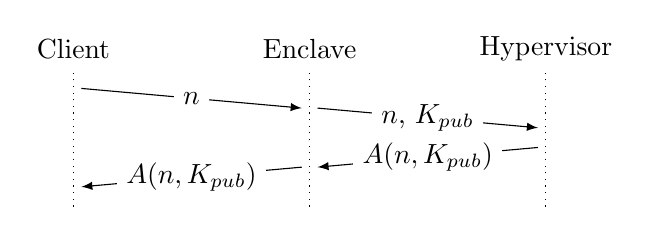
\begin{tikzpicture}[node distance=20pt]

  %               x,y      x,y
  \draw [dotted] (0,0) -- (0,1.75);
  \draw [dotted] (3,0) -- (3,1.75);
  \draw [dotted] (6,0) -- (6,1.75);

  \node at (0,2) {Client};
  \node at (3,2) {Enclave};
  \node at (6,2) {Hypervisor};

  \draw [-latex]
        (0.1, 1.5) -- (2.9, 1.25) node [midway, fill=white, text centered]
        { $n$ };

  \draw [-latex]
        (3.1, 1.25) -- (5.9, 1) node [midway, fill=white, text centered]
        { $n$, $K_{pub}$ };

  \draw [-latex]
        (5.9, 0.75) -- (3.1, 0.5) node [midway, fill=white, text centered]
        { $A(n, K_{pub})$ };

  \draw [-latex]
        (2.9, 0.5) -- (0.1, 0.25) node [midway, fill=white, text centered]
        { $A(n, K_{pub})$ };

\end{tikzpicture}

  \caption{Clients provide a nonce $n$ when requesting an attestation document
  from the enclave.  The enclave asks its hypervisor for the attestation
  document $A$, providing the client's nonce and its public key $K_{pub}$.  The
  hypervisor responds with the attestation document $A(n, K_{pub})$, which the
  enclave forwards to the client.}%
  \label{fig:attestation}
\end{figure}

{\bf First}, the attestation document is signed by the AWS root CA whose public
key (which serves as the root of trust) is known to all parties.  This prevents
all parties except Amazon from issuing malicious attestation documents.

{\bf Second}, the challenge nonce is part of the attestation document.  This
prevents adversaries from replaying old attestation documents.

{\bf Third}, the fingerprint of the enclave's X.509 certificate from the TLS
session is part of the attestation document.  This prevents adversaries from
intercepting the secure channel.

{\bf Fourth}, the enclave's image ID is identical to the image ID that the
client compiled locally.  This prevents adversaries from tricking clients into
talking to a malicious enclave.

Only if all four conditions hold is the client convinced that it is talking to
an enclave running the previously-audited code \emph{and} that the secure
channel is terminated inside the enclave.  Note that the EC2 host is able to
intercept the secure channel with its own CA-signed certificate but clients will
only trust the EC2 host if (and only if) it can present an attestation document
that is valid for the enclave image, which it can't because it is unable to
spoof the AWS root CA signature that authenticates the attestation document.
The only way for the EC2 host to obtain such an attestation document is to spawn
an enclave that runs the exact code that the client is expecting---and it
already does exactly that.  Now that the client has established a trust
relationship with the enclave, it is ready to reveal sensitive information to
the enclave.

\subsubsection{Syncing key material among enclaves}%
\label{sec:sync}

Enclaves are sealed at runtime, preventing anyone (including both Amazon and the
service provider) from extracting key material that was generated inside the
enclave.  While a desirable property, this complicates horizontal scaling.  If a
single enclave proves unable to handle traffic load, one must scale horizontally
by starting new enclaves.  In some applications, it is unacceptable for each
enclave to use distinct key material.  Instead, enclaves must synchronize their
key material to appear to the outside world like a single machine.  While it is
possible to accomplish key synchronization using tools like the AWS key
management service (KMS),\footnote{One could encrypt the keys using a KMS policy
that dictates that only enclaves are allowed to decrypt it, and store the
encrypted key in a location that all enclaves can access, e.g., an S3 bucket.}
we refrain from using KMS because users currently cannot verify that a
KMS ``key policy'' is truly immutable.  We therefore devise a novel,
user-verifiable protocol that enables key synchronization without having to rely
on external services.

We solve this problem in two steps: \emph{discovery}, followed by
\emph{synchronization}.  First, enclaves must be able to discover each other,
i.e., learn each other's IP addresses.  Then, enclaves can establish connections
with each other and initiate key synchronization.  Our protocol dictates that
when a new enclave bootstraps, it first tries to discover already-existing
enclaves.  If there are none, the enclave knows that it is the ``origin''
enclave.  It then generates new key material that it will share with future
enclaves.  If however it discovers other enclaves, the new enclave establishes a
connection with another, randomly-chosen enclave and initiates key
synchronization.  Crucially, key material is only shared after \emph{mutual
attestation}, i.e., the origin and new enclaves verify each other, and exchange
key material only if remote attestation succeeds.  Key synchronization happens
in three steps, as illustrated in Figure~\ref{fig:key-synchronization}.

\begin{figure}[t]
  \centering
  \begin{tikzpicture}[node distance=20pt]

  \node [draw,
         align=center,
         fill=black!20!gray,
         minimum height=70pt] (enclave2) {\color{white}New\\\color{white}enclave};
  \node [draw,
         align=center,
         fill=black!20!gray,
         minimum height=70pt,
         right=140pt of enclave2] (enclave1) {\color{white}Original\\\color{white}enclave};
  \node [draw,
         densely dotted,
         label=below left:Virtual network,
         fit=(enclave1) (enclave2)] {};

  \node [draw,
         above=of enclave2] (resolver) {DNS resolver};

  % New enclave discovers existing enclaves via DNS.
  \draw [-latex] ([xshift=3pt]enclave2.north) -- ([xshift=3pt]resolver.south)
        node [midway, right] {Request DNS SRV records};
  \draw [latex-] ([xshift=-3pt]enclave2.north) -- ([xshift=-3pt]resolver.south);

  % New enclave asks original enclave for nonce.
  \draw [-latex] ([yshift=30pt]enclave2.east) -- ([yshift=25pt]enclave1.west)
        node [midway, fill=white, align=center]
        {\emph{Request nonce}};
  \draw [latex-] ([yshift=15pt]enclave2.east) -- ([yshift=20pt]enclave1.west)
        node [midway, fill=white, align=center]
        {$\textrm{nonce}_o$};

  % New enclave asks for keys.
  \draw [-latex] (enclave2.east) -- ([yshift=-5pt]enclave1.west)
        node [midway, fill=white, align=center]
        {\emph{Request keys}\\$A_{n}(\textrm{nonce}_o, K_n, \ \textrm{nonce}_n$)};

  \draw [latex-] ([yshift=-30pt]enclave2.east) -- ([yshift=-25pt]enclave1.west)
        node [midway, fill=white, align=center]
        {$A_{o}(\textrm{nonce}_n, \textsf{Enc}(K_n, s))$};

\end{tikzpicture}

  \caption{When a new enclave bootstraps, it discovers existing enclaves by
    obtaining the DNS SRV record for its own, hard-coded FQDN.  The enclave then
    initiates key synchronization by first requesting a nonce.  Then, the new
    enclave requests the origin enclave's key material by submitting its own
    attestation document, followed by receiving the origin enclave's attestation
    document, which contains encrypted key material.}
  \label{fig:key-synchronization}
\end{figure}

\textbf{First}, once a new enclave is spun up, it queries the DNS SRV record of
the FQDN that is hard-coded in the enclave, e.g., example.com.  The DNS resolver
will return the record, containing a list of enclaves that are already running
and initialized.  The new enclave picks a random enclave from the list and
initiates key synchronization.  Running Nitro Enclaves as part of Kubernetes
can handle DNS record generation automatically.

\textbf{Second}, the new enclave asks the existing enclave for a random nonce,
$\textrm{nonce}_o$.  Both enclaves cache $\textrm{nonce}_o$ for one minute to
mitigate denial-of-service attacks.

\textbf{Third}, the new enclave now requests the key material from the existing
enclave.  As part of the request, it provides its attestation document that
contains $\textrm{nonce}_o$ (to prove freshness to the existing enclave);
$\textrm{nonce}_n$ (the existing enclave is expected to add this nonce to its
attestation document); and $K_n$ (a NaCl public key~\cite{nacl} to which the key
material should be encrypted).  Upon receipt of the new enclave's attestation
document, the existing enclave verifies the attestation document's signature and
ensures that the new enclave is running the same code, i.e., the image ID that
uniquely identifies the enclave image is identical.  Once the existing enclave
is convinced that it is dealing with a genuine new enclave, it creates an
attestation document by including $\textrm{nonce}_n$ (to prove freshness to the
new enclave) and $\textsf{Enc}(K_n, s)$---the key material $s$ is encrypted
using the public key that the new enclave provided in the request.  Finally, the
new enclave verifies the attestation document, decrypts the key material, and
uses it to finish bootstrapping.

% Security considerations.
The security of key synchronization is paramount.  We take advantage of mutual
remote attestation to protect the key material.  As an optional layer of
defense-in-depth, synchronization should be configured to use a private network,
which prevents arbitrary Internet hosts from talking to the synchronization
endpoint.  While not required, we recommend running enclaves as part of
Kubernetes because it provides a private network that is shared by enclaves.

In their 2022 USENIX Security paper, Chen and Zhang present MAGE, a protocol
that allows enclaves to mutually verify each other without relying on a trusted
third party~\cite{Chen2022a}.  We could have built key synchronization on top of
MAGE but found that our setting is considerably simpler because only
\emph{identical} enclaves request each other's key material, eliminating the
need for the more flexible---but also more complex---MAGE protocol.

\subsubsection{Side-channel attacks}%
\label{sec:side-channels}

The enclave's EC2 host cannot see \emph{what} clients send to the enclave but it
can see \emph{how much} clients send and \emph{how long} it takes the enclave to
process data.  The EC2 host can exploit these side channels to learn more about
the client's confidential information and computation.  While such side channels
must be avoided, \tool{} is not the place to do so.  Instead, it is the enclave
application developer's responsibility to identify and address this class of
attacks, e.g., by implement constant-time processing.

\subsubsection{Ingesting secrets}%
\label{sec:secrets}

A key design requirement of \tool{} is that users must be able to audit the
enclave application's code.  The service provider is therefore unable to hide
any software configuration (e.g., confidential API keys) from the user.  Service
providers can work around this shortcoming by exposing an authenticated HTTP
handler that takes as input arbitrary data that updates the enclave's state.
Consider a system that takes as input client IP addresses, anonymizes them, and
forwards the anonymized addresses to a back end.  The service provider now wants
to compare submitted IP addresses to a confidential deny list.  If however the
deny list is hard-coded in the publicly available enclave application, it is
readily visible to anyone.  The service provider can solve this problem by
adding to the enclave application a new HTTP handler that takes as input the
confidential data it seeks to protect from the users' eyes.  Once the enclave is
running, the service provider loads the confidential deny list.  To prevent
users from submitting bogus data, the endpoint must be authenticated.  One
could accomplish this by hard-coding the service provider's public key in the
enclave application, and only accepting deny lists that carry a valid signature.
Another possibility is to expose this endpoint only to the EC2 host, so only the
service provider has access to it.  We provide an example of this in
Section~\ref{sec:vct}.

This technique for ingesting secrets is flexible---so flexible, in fact, that
the service provider could abuse it to ingest code at runtime, which would
nullify the enclave's verifiability requirement.  Vigilant users would never
trust an enclave whose code can change at runtime.  We therefore argue that an
HTTP handler for the purpose of ingesting secrets must be constrained so that
only well-defined data of a certain type (like a deny list) can be ingested.
